% This is "sig-alternate.tex" V2.1 April 2013
% This file should be compiled with V2.5 of "sig-alternate.cls" May 2012
%
% This example file demonstrates the use of the 'sig-alternate.cls'
% V2.5 LaTeX2e document class file. It is for those submitting
% articles to ACM Conference Proceedings WHO DO NOT WISH TO
% STRICTLY ADHERE TO THE SIGS (PUBS-BOARD-ENDORSED) STYLE.
% The 'sig-alternate.cls' file will produce a similar-looking,
% albeit, 'tighter' paper resulting in, invariably, fewer pages.
%
% ----------------------------------------------------------------------------------------------------------------
% This .tex file (and associated .cls V2.5) produces:
%       1) The Permission Statement
%       2) The Conference (location) Info information
%       3) The Copyright Line with ACM data
%       4) NO page numbers
%
% as against the acm_proc_article-sp.cls file which
% DOES NOT produce 1) thru' 3) above.
%
% Using 'sig-alternate.cls' you have control, however, from within
% the source .tex file, over both the CopyrightYear
% (defaulted to 200X) and the ACM Copyright Data
% (defaulted to X-XXXXX-XX-X/XX/XX).
% e.g.
% \CopyrightYear{2007} will cause 2007 to appear in the copyright line.
% \crdata{0-12345-67-8/90/12} will cause 0-12345-67-8/90/12 to appear in the copyright line.
%
% ---------------------------------------------------------------------------------------------------------------
% This .tex source is an example which *does* use
% the .bib file (from which the .bbl file % is produced).
% REMEMBER HOWEVER: After having produced the .bbl file,
% and prior to final submission, you *NEED* to 'insert'
% your .bbl file into your source .tex file so as to provide
% ONE 'self-contained' source file.
%
% ================= IF YOU HAVE QUESTIONS =======================
% Questions regarding the SIGS styles, SIGS policies and
% procedures, Conferences etc. should be sent to
% Adrienne Griscti (griscti@acm.org)
%
% Technical questions _only_ to
% Gerald Murray (murray@hq.acm.org)
% ===============================================================
%
% For tracking purposes - this is V2.0 - May 2012

\documentclass{sig-alternate-05-2015}

\usepackage{listings}
\usepackage{float}

\newcommand{\eg}[0]{{\em e.g., }}
\newcommand{\etc}[0]{{\em etc. }}
\newcommand{\ie}[0]{{\em i.e., }}

\begin{document}

\CopyrightYear{2016} 
\setcopyright{acmcopyright}
\conferenceinfo{SIGIR '16,}{July 17-21, 2016, Pisa, Italy}
\isbn{978-1-4503-4069-4/16/07}\acmPrice{\$15.00}
\doi{http://dx.doi.org/10.1145/2911451.2911536}

\title{When a Knowledge Base Is Not Enough: Question Answering over Knowledge Bases with External Text Data}


%
% You need the command \numberofauthors to handle the 'placement
% and alignment' of the authors beneath the title.
%
% For aesthetic reasons, we recommend 'three authors at a time'
% i.e. three 'name/affiliation blocks' be placed beneath the title.
%
% NOTE: You are NOT restricted in how many 'rows' of
% "name/affiliations" may appear. We just ask that you restrict
% the number of 'columns' to three.
%
% Because of the available 'opening page real-estate'
% we ask you to refrain from putting more than six authors
% (two rows with three columns) beneath the article title.
% More than six makes the first-page appear very cluttered indeed.
%
% Use the \alignauthor commands to handle the names
% and affiliations for an 'aesthetic maximum' of six authors.
% Add names, affiliations, addresses for
% the seventh etc. author(s) as the argument for the
% \additionalauthors command.
% These 'additional authors' will be output/set for you
% without further effort on your part as the last section in
% the body of your article BEFORE References or any Appendices.

\numberofauthors{2} %  in this sample file, there are a *total*
% of EIGHT authors. SIX appear on the 'first-page' (for formatting
% reasons) and the remaining two appear in the \additionalauthors section.
%
\author{
% 1st. author
\alignauthor
Denis Savenkov\\
       \affaddr{Emory University}\\
       \email{dsavenk@emory.edu}
% 2nd. author
\alignauthor
Eugene Agichtein\\
		\affaddr{Emory University}\\
       \email{eugene@mathcs.emory.edu}
}
% There's nothing stopping you putting the seventh, eighth, etc.
% author on the opening page (as the 'third row') but we ask,
% for aesthetic reasons that you place these 'additional authors'
% in the \additional authors block, viz.
%\additionalauthors{Additional authors: John Smith (The Th{\o}rv{\"a}ld Group,
%email: {\texttt{jsmith@affiliation.org}}) and Julius P.~Kumquat
%(The Kumquat Consortium, email: {\texttt{jpkumquat@consortium.net}}).}
%\date{30 July 1999}
% Just remember to make sure that the TOTAL number of authors
% is the number that will appear on the first page PLUS the
% number that will appear in the \additionalauthors section.

\maketitle
\begin{abstract}

One of the major challenges for knowledge base question answering systems (KBQA) is to translate a natural language question to knowledge base (KB) entities and predicates.
Previous systems have used a limited amount of training data to learn a lexicon that is later used for question answering.
This approach does not make use of other potentially relevant text data, outside the KB, which could enrich the available information.
We introduce a new system, Text2KB, that connects a KB with external text. Specifically, we revisit different phases in the KBQA process and demonstrate that text resources improve question interpretation, candidate generation and ranking.
Starting with the best publicly available system, Text2KB utilizes web search results, community question answering and general text document collection data, to detect question topic entities and enrich the features of the candidates derived from the KB.
Text2KB significantly improves on the initial KBQA system, and reaches the best known state of the art performance on a popular WebQuestions knowledge base question answering dataset.
The results and insights developed in this work are both practically useful, and can guide future efforts on combining textual and structured KB data for question answering.


\end{abstract}


% The code below should be generated by the tool at
% http://dl.acm.org/ccs.cfm
% Please copy and paste the code instead of the example below. 
%
%\begin{CCSXML}
%<ccs2012>
% <concept>
%  <concept_id>10010520.10010553.10010562</concept_id>
%  <concept_desc>Computer systems organization~Embedded systems</concept_desc>
%  <concept_significance>500</concept_significance>
% </concept>
% <concept>
%  <concept_id>10010520.10010575.10010755</concept_id>
%  <concept_desc>Computer systems organization~Redundancy</concept_desc>
%  <concept_significance>300</concept_significance>
% </concept>
% <concept>
%  <concept_id>10010520.10010553.10010554</concept_id>
%  <concept_desc>Computer systems organization~Robotics</concept_desc>
%  <concept_significance>100</concept_significance>
% </concept>
% <concept>
%  <concept_id>10003033.10003083.10003095</concept_id>
%  <concept_desc>Networks~Network reliability</concept_desc>
%  <concept_significance>100</concept_significance>
% </concept>
% </ccs2012>  
%\end{CCSXML}

%\ccsdesc[500]{Computer systems organization~Embedded systems}
%\ccsdesc[300]{Computer systems organization~Redundancy}
%\ccsdesc{Computer systems organization~Robotics}
%\ccsdesc[100]{Networks~Network reliability}
%
% End generated code
%
%
%  Use this command to print the description
%
%\printccsdesc

% We no longer use \terms command
%\terms{Theory}

% \keywords{ACM proceedings; \LaTeX; text tagging}

\section{Introduction}
\label{section:intro}
Traditionally question answering systems used text document collections to retrieve passages relevant to a question and to extract candidate answers \cite{Vrandecic:2014:WFC:2661061.2629489}.
Unfortunately, a paragraph of text encodes a very limited amount of information about answer candidates and predictions has to be used instead, \eg most of the systems estimate candidate answer entity type to match against the expected type inferred from the question text.
On the other hand, modern large scale open-domain knowledge bases, such as dbPedia \cite{auer2007dbpedia}, Freebase \cite{Bollacker:2008:FCC:1376616.1376746} and WikiData \cite{Vrandecic:2014:WFC:2661061.2629489} store a vast amount of general knowledge about different kinds of entities.
This information, encoded as \texttt{[subject, predicate, object]} RDF triples, can be effectively queried using structured query languages, such as SPARQL.
Of course, regular users would rather prefer to ask natural language questions.
Translation of text questions into structured query languages is very challenging for a number of reasons: complexity of a KB schema, variability of natural language and knowledge representation \etc
For example, Figure \ref{fig:example_sparql} gives a SPARQL query that retrieves the answer to a relatively easy question \textit{``who is the current president of the dominican republic in 2010?''}.
% The same information can be asked in many different ways, for example: \textit{``who is the dominican republic president in 2010?''}, or \textit{``who was the leader of the dominican republic in 2010?''} \etc

\begin{figure*}
\centering
\begin{lstlisting}[frame=single]
PREFIX : <http://rdf.freebase.com/ns/>
SELECT DISTINCT ?name {
   :m.027rn :government.governmental_jurisdiction.governing_officials ?gov_position .
   ?gov_position :government.government_position_held.basic_title :m.060c4 .
   ?gov_position :government.government_position_held.office_holder ?president .
   ?gov_position :government.government_position_held.from ?from_date .
   ?gov_position :government.government_position_held.to ?to_date .
   FILTER (
       xsd:date(?from_date) <= "2010"^^xsd:date AND
       xsd:date(?to_date) >= "2010"^^xsd:date
   )
   ?president :type.object.name ?name
}
\end{lstlisting}
\caption{SPARQL query that retrieves the answer to the query \textit{``who is the current president of the dominican republic in 2010?''}}
\label{fig:example_sparql}
\end{figure*}

\begin{figure}
\centering
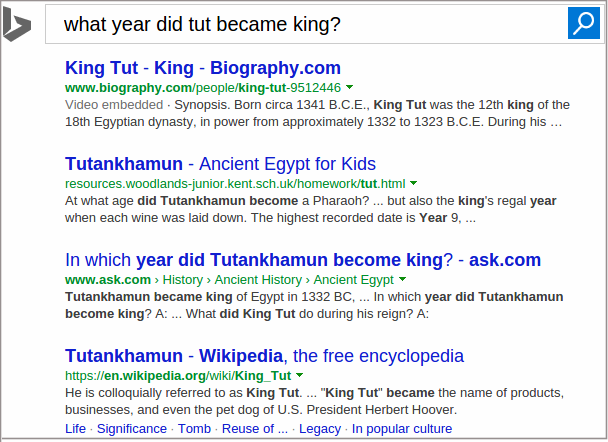
\includegraphics[width=0.5\textwidth]{img/web_search_entitylink}
\caption{Search results for the question ``what year did tut became king?''}
\label{fig:web_search_entitylink}
\end{figure}

The first problem that a KBQA system is facing is question entity identification.
The performance of the whole system greatly depends on this stage \cite{yao-scratch-qa-naacl2015}, because it seeds the answer candidate search process.
Question text is often quite short, may contain typos and other problems, that complicate question entity identification.
Existing approaches are usually based on dictionaries that contain entity names, aliases and some other phrases, which were used to refer to entities \cite{SPITKOVSKY12.266}.
These dictionaries are often noisy and incomplete, \eg to answer the question \textit{``what year did tut became king?''} a system needs to detect a mention \textit{``tut''}, which refers to the entity \textit{``Tutankhamun''}.
A mapping \textit{tut $\rightarrow$ ``Tutankhamun''} is missing in the dictionary used by one of the state of the art systems and therefore it couldn't answer this question correctly.
Instead of increasing the dictionary size we propose to use web search results to find variations of question entity names, which can be easier to link to a KB.
This idea was used for entity linking in web search queries \cite{SMAPH_ERD:2014}, which was given as one of the tracks on the Entity Recognition and Disambiguation Challenge 2014\footnote{http://web-ngram.research.microsoft.com/ERD2014/}.
Figure \ref{fig:web_search_entitylink} presents web search results for the query \textit{``what year did tut became king?''}, which shows that indeed many documents mention the full name, which can easily be mapped to a KB entity.

After question entities have been identified the next step is to explore their neighborhood and build structured queries as candidate answers.
A query addresses one or multiple KB predicates, which should be somehow related to words and phrases in the question and systems try score these mappings in order to select the best answer.
Existing knowledge base question answering approaches \cite{ACCU:2015,Berant:EMNLP13,berant2014semantic,berant2015imitation,BordesCW14:emnlp,yao2014freebase} rely on some kind of a lexicon, which is learned from manually labeled training data and supported by some additional resources, such as question paraphrases \cite{berant2014semantic} and weakly labeled sentences from a large text collection \cite{yao2014information}.
However, given the fact that manually labeled training data is very limited, such lexicons do not cover thousands of different predicates present in a KB.
By our estimate in a popular WebQuestions KBQA dataset answers to $\sim$5.5\% of test questions (112 out of 2032) involve a predicate, that doesn't appear in the training set.
For example, an RDF triple \texttt{[Bigos, food.dish.type\_of\_dish1, Stew]} answers a test question \textit{``what are bigos?''}, but there are no questions from the training set that are answered using the same predicate.
In addition, even if training set contains an example targeting a particular KB predicate, the lexicon might not cover all the other possible ways the same information can be asked about.
For example, test question \textit{``who is the woman that john edwards had an affair with?''} is similar in meaning and is answered with a similar query as a training set question \textit{``who did jon gosselin cheat with?''}, but the word \textit{affair} isn't used in the training set.
On the other hand, traditional text-based question answering systems benefit from the redundancy with which the same information is stated in many different ways in many documents \cite{Lin:2007:EPU:1229179.1229180}.
This increases the chances of a good lexical match between a question and answer statements, which makes even some relatively simple counting-based techniques quite effective \cite{brill2002analysis}.
We propose to borrow some ideas from text-based question answering and enrich the representation of candidate structured queries with additional text documents and fragments, that can help to select the best answer.
For example, the right part of the Figure \ref{fig:model} shows web search results, community question answering page and text fragments mentioning pairs of entities, that can clearly be useful to answer the question about John Edwards' affair.

\subsection{Contributions}

Our main contributions in this work are three-fold:
\begin{itemize}
\item a novel ``hybrid'' knowledge base question answering system, which uses both structured data from a knowledge base and unstructured natural language resources connected via entity links. Section \ref{section:method} describes the architecture of our system, and Section \ref{section:eval} shows that this fusion improves the performance of a state of the art KBQA system.
\item novel data sources for knowledge base question answering. Entity linking allows us to connect test resources with a KB. We explore three different types of text data, that is useful for KBQA: web search results (Section \ref{section:method:web}), Community Question Answering data (Section \ref{section:method:cqa}) and entity pairs language model based on a large text corpus (Section \ref{section:method:clueweb}).
\item evaluation and analysis. We evaluate the performance of our system on a popular WebQuestions dataset and demonstrate that using additional text resources we can improve the quality of knowledge base question answering (Section \ref{section:eval}). In addition, we conduct an extensive analysis of the system and suggest directions for future research (Section \ref{section:analysis}).
\end{itemize}

% -------------------------------------------

%There are many problems in KBQA:
%\begin{itemize}
%\item lexical variations, we can call the same thing in million ways
%\item representation variation - similar data can be represented in multiple ways, e.g. capital of the state in Australia location.australian\_state.capital\_city, while in the US you will have totally different predicate. HOWEVER, these are old predicate and marked deprecated. There is another predicate that should be the same for both cases.
%\item Incomplete, some data is simply missing or details are not present. E.g. who is the woman that john edwards had an affair with?, there is a triple that says that he had sexual relationships with Rielle Hunter, but there is no details...
%\item Related to the previous - many predicates are simply not present. There is something related, but not exactly what is asked about. Example: where did andy murray started playing tennis? We can find the answer entity, but the triple won't say that he started playing there.
%\end{itemize}

%In \cite{Sun:2015:ODQ:2736277.2741651} authors report pretty low score for Sempre on TREC and Bing QA datasets.

% Questions and corresponding answers are often expressed differently and researchers in question answering studied different ways to bridge this lexical gap, \eg using translation models \cite{Murdock:2005:TMS:1220575.1220661} and distributional semantics \cite{yu2014deep}.




\section{Knowledge Base Question Answering: an Overview}
\label{section:baseline}
In this section, we overview the existing approaches to Knowledge Base Question Answering (KBQA), as our approach, described in the next section, builds upon and extends some of these efforts. 

Recently, KBQA systems have converged to two major approaches: {\em semantic parsing}, and {\em information extraction} (IE) \cite{yao2014freebase}.
The former focuses on question understanding, and attempts to parse the sentences into a semantic representation, \eg logical forms \cite{Berant:EMNLP13,berant2014semantic,berant2015imitation}. IE approaches \cite{ACCU:2015,yih2015semantic,yao2014information} are based on identifying \textit{topical entities} in the question, and then, using pre-defined templates for mapping the question to predicates, explore the neighborhood of these entities in a KB.
Theoretically, semantic parsing-based systems would be capable of generating any required queries, and would apply to any question, seen or unseen in training, whereas the template-based approach is less likely to generalize. In practice, however, answers to most of the questions lie within two edge traversals in a KB, making the template (``information extraction''-based) approaches quite effective.

Interestingly, one of the reasons for recent resurgence of interest in KBQA can be credited to creation of the WebQuestions dataset \cite{Berant:EMNLP13}, which is large enough to allow both comprehensive evaluation, and training machine learning methods.
Thus, the performance of KBQA systems has quickly improved, with the current state of the art systems using the IE approach, with sophisticated ranking and matching postprocessing \cite{yih2015semantic}.
In this work, we chose to extend an existing informtion extraction KBQA system -- Aqqu \cite{ACCU:2015} -- which achieves one of the highest scores among publicly available systems.
However, as we will show, our approach is general and can be incorporated into other IE-based systems as well.

%One of the most popular benchmark datasets for knowledge base question answering is WebQuestions \cite{Berant:EMNLP13}, which has attracted a lot of attention recently and as a result the performance increased from 0.357 \cite{Berant:EMNLP13} to 0.525 \cite{yih2015semantic} in average F1 over test questions.
%The dataset is based on Freebase, which has been recently shut down\footnote{https://goo.gl/SZC3tg}.
%The shutdown of Freebase means that it will no longer be extended, but all the data will be available and it will be merged with WikiData\footnote{https://www.wikidata.org/}.
%Therefore, future datasets should probably use different reference KB, but there is no problem in using Freebase for experiments on existing benchmarks, such as WebQuestions.
%We should also stress, that the proposed approach isn't tied to Freebase and can be applied for question answering over dbPedia, WikiData or other knowledge bases.

%The focus of this work is on the fusion between structured data in the KB and unstructured text data.
%Therefore, we chose to extend an existing KBQA system: Aqqu \cite{ACCU:2015}.
%It follows an information extraction approach to KBQA and achieves one of the highest scores among publicly available systems.
%However, our approach can be incorporated into other systems as well.

We will first describe an information extraction approach to KBQA in more detail using Aqqu -- our baseline system -- as an example.
In Section \ref{section:method} we present our system Text2KB, which extends this approach by incorporating external text-based data on various stages of the question answering process.

\begin{figure*}[!ht]
\centering
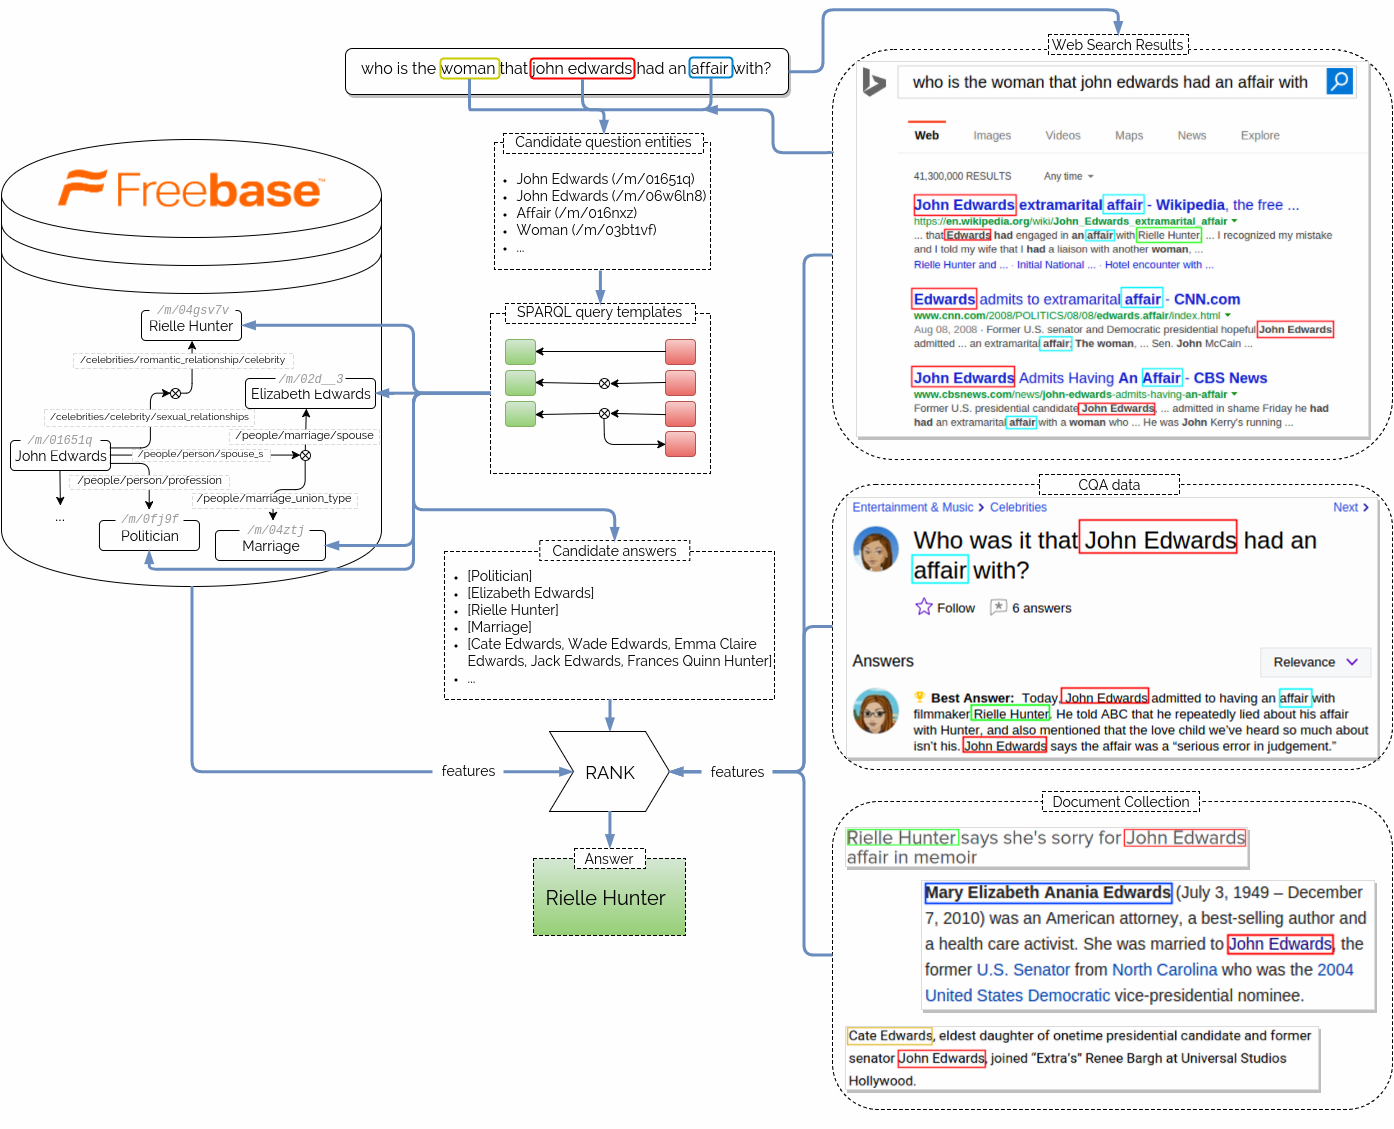
\includegraphics[width=0.9\textwidth]{img/Text2KB_model}
\caption{The architecture of our Text2KB Question Answering system}
\label{fig:model}
\end{figure*}


\subsection{The Aqqu KBQA system}
\label{sec:baseline:aqqu}

First, a KBQA system needs to identify question entities, which are used as sources for the answer search process.
For concreteness, consider a question from the WebQuestions dataset \textit{``who is the woman that john edwards had an affair with?''}.
In this example, entity \texttt{John Edwards} with Freebase mid \texttt{/m/01651q} is the main question entity.
However, Freebase contains millions of entities and it's often hard to identify the topical ones (\eg entities \texttt{Woman} and \texttt{Affair} are also present in Freebase), or to disambiguate and choose between \texttt{John Edwards} a politician (\texttt{/m/01641q}), \texttt{John Edwards} an American racing driver (\texttt{/m/06zs089}) and other people with the same name.
% There is even an entity with the name ``\texttt{had an affair with}''\footnote{http://www.freebase.com/m/0c0n01x}.
Aqqu considers all spans of question words under certain conditions on part of speech tags and uses a dictionary of names, aliases and anchor texts \cite{SPITKOVSKY12.266} to map phrases to potential entities.
Most recent systems, including Aqqu, don't disambiguate entities at this stage and keep a set of candidates along with some information about their popularities (number of triples in the KB, or number of mentions in the collection) and mention scores $p(entity| mention\ text)$.

On the next stage, SPARQL query candidates are generated by exploring the neighborhood of the question topical entities using a predefined set of query templates.
Each query template has question entities, predicate and answer placeholders.
Majority of the answers in WebQuestions dataset can be covered by just 3 templates (q\_entity - question entity, a\_entity - answer entity, cvt\_node - Freebase mediator node, which represent tuples with more than 2 arguments):

\begin{lstlisting}[frame=single,basicstyle=\small]
SELECT DISTINCT ?a_entity {
   <q_entity> <predicate> ?a_entity .
}
\end{lstlisting}

\vspace{-0.25cm}
\begin{lstlisting}[frame=single,basicstyle=\small]
SELECT DISTINCT ?a_entity {
   <q_entity> <predicate_1> ?cvt_node .
   ?cvt_node <predicate_2> ?a_entity .
}
\end{lstlisting}

\vspace{-0.25cm}
\begin{lstlisting}[frame=single,basicstyle=\small]
SELECT DISTINCT ?a_entity {
   <q_entity_1> <predicate_1> ?cvt_node .
   ?cvt_node <predicate_2> <q_entity_2> .
   ?cvt_node <predicate_3> ?a_entity .
}
\end{lstlisting}

The first template retrieves a set of entities that are directly connected to the given question entity via a certain predicate.
The second template accounts for the presence of a mediator node, that groups together arguments of a multi-argument relation.
And the last template looks for cases, when a question also mentions another argument of a multi-argument relation, \eg \texttt{Captain Kirk} and \texttt{Star Trek} for the question \textit{``who played captain kirk in star trek movie?''}.

Each query candidate is represented with a set of features, that includes the scores for linked question entities, various scores for matching between question term n-grams and query predicates, the size of the results list, \etc \cite{ACCU:2015}.
The final stage of the question answering process is filtering and ranking, using a random forest model, built on the training part of the WebQuestions dataset.

\subsection{Basic system extensions}
\label{sec:baseline:extensions}
Before introducing our text-based improvements, described in Section~\ref{section:method}, we introduced some basic improvements to the original Aqqu system.
First, we noticed that since Aqqu does not use information about answer entity Freebase types, in many cases it returns an answer that is incompatible with the question: \eg state instead of county \etc
Therefore, we a trained a model to return a score, measuring a compatibility between the question and answer entities, based on the entity notable types and question uni- and bigrams as features, similar to Aqqu's relations score model.
A second extension introduced a new date range query template, which helps to solve the cases like \textit{``what team did david beckham play for in 2011?''}, where we need to look at the ranges of dates to figure out in which range does the specified date falls.

\begin{lstlisting}[frame=single,basicstyle=\small]
SELECT DISTINCT ?a_entity {
   <q_entity_1> <predicate_1> ?cvt_node .
   ?cvt_node <from_predicate> ?date_from .
   ?cvt_node <to_predicate> ?date_to .
   ?cvt_node <predicate_2> ?a_entity .
   FILTER ( <question_date> >= ?date_from AND
            <question_date> <= ?date_to )
}
\end{lstlisting}

%We also experimented with an additional template, which filters out lists by the entity notable types.



\section{Text2KB: Incorporating Text Data into KBQA}
\label{section:method}

\subsection{Baseline method}
Our approach is based on the system proposed in \cite{ACCU:2015}.

\subsubsection{Extensions}
We implemented a couple of extensions of the baseline system.

\begin{itemize}
\item date range based filters
\item notable types based filters
\item notable types based model, used as a feature
\end{itemize}

\subsection{Unstructured data for KBQA}

\subsubsection{Text data in KB}
We use entity descriptions to generate a set of features for candidate answers.

\subsubsection{Web search results}
We issue question to a web search using Bing Web Search API\footnote{API URL should go here}.
Returned documents and snippets are used by our question answering system.

\begin{itemize}
\item Entity linking from snippets, similar to \cite{SMAPH_ERD:2014}.
\item Textual and entity similarity features based on search results documents and snippets
\end{itemize}

\subsubsection{Community Question Answering collection}
Using a collection of question-answer pairs from Yahoo! Answers we annotated questions and answers with entities and relations between pairs of entities.
This approach follows distant supervision approach for relation extraction \cite{savenkov-EtAl:2015:SRW}.
Pairs of question words and relations are used to generate features.

\subsubsection{Entity-linked collection of documents}
We take ClueWeb12 and use existing entity links generated by Google to build an index from entity pair to phrases, that occur around these entities in the collection.
This data is used to generate features for candidates.

\subsubsection{Wikipedia profile}
It would be nice to have Wikipedia pages for entities and use something like SDM score or something else as feature.

\section{Evaluation}
\label{section:eval}

We followed the standard evaluation procedure for the WebQuestions dataset and used existing train-test splits for reporting our results.
The benchmark uses average F1 score, which gives a partial credit to list answers that are not equal but overlap with the correct answer.
We also report average precision and recall, as well as an F1 score of average precision and recall.
The results of existing approaches, our baseline and Text2KB systems is presented in Table \ref{table:webquestions_results}.

\begin{table*}
\centering
\caption{Performance of the Text2KB system on WebQuestions dataset}
\label{table:webquestions_results}
\begin{tabular}{| p{5cm} | p{1.5cm} | p{1.5cm} | p{1.5cm} | p{1.5cm} | }
\hline
System & avg Recall & avg Precision & F1 of avg Prec and Recall & avg F1 \\
\hline
SemPre \cite{Berant:EMNLP13} & 0.413 & 0.480 & 0.444 & 0.357\\
Subgraph Embeddings \cite{BordesCW14:emnlp} & - & - & 0.432 & 0.392\\
ParaSemPre \cite{berant2014semantic} & 0.466 & 0.405 & 0.433 & 0.399\\
Jacana \cite{yao2014information} & 0.458 & 0.517 & 0.486 & 0.330\\
Kitt AI \cite{yao-scratch-qa-naacl2015} & 0.545 & 0.526 & 0.535 & 0.443\\
AgendaIL \cite{berant2015imitation} & 0.557 & 0.505 & 0.530 & 0.497\\
STAGG \cite{yih2015semantic} & 0.607 & 0.528 & 0.565 & 0.525\\
STAGG (no duplicates\footnote{An answer of the STAGG system may contain duplicate entities, which are double counted by the evaluation script}) \cite{yih2015semantic} & 0.6067 & 0.5263 & 0.5634 & 0.5234 \\
\hline
Accu (baseline) \cite{ACCU:2015} & 0.604 & 0.498 & 0.546 & 0.494\\
% DIDN'T HAVE TIME TO IMPLEMENT THIS.
% Text-only baseline & & & & \\
Our system: Text2KB & 0.6354 & 0.5059 & 0.5633 & 0.5223 \\
\hline
Text2KB + STAGG & 0.5976 & 0.5343 & 0.5641 & 0.5320 \\
Text2KB + STAGG (oracle) & 0.7144 & 0.5904 & 0.6465 & 0.6056 \\
\hline
\end{tabular}
\end{table*}

As we can see, Text2KB significantly improves over the baseline system and reaches the current best published result - STAGG \cite{yih2015semantic}.
However, we believe that this system will also benefit from the ideas of our work.
To support this claim we combined results of STAGG and Text2KB systems using a simple heuristic: we prefer STAGG result when its answer length is shorter than Text2KB.
This heuristic is inspired by the fact, that STAGG has a filtering stage, that filters out result lists based on some criteria, \ie gender, entity type, \etc
However, there is still a room for improvement if the combination is done inside a system, because the errors of STAGG and Text2KB differ, and if we use an oracle, which chooses an answer with the higher F1 score, we can achieve an average F1 of 0.6056.

We also evaluated both STAGG and Text2KB on 112 questions, where the correct answer is retrieved via a predicate, that weren't used in the positive training examples.
These questions are harder to answer, and the average F1 score of Text2KB is 0.1640 versus 0.1199 for STAGG.
This gives some anecdotal evidence, that by incorporating external text resources we were able to answer these questions slightly better, how these difference isn't statistically significant according to paired t-test (p-value 0.16).

\subsection{Ablation Study}

To study individual effects of different components we made an ablation study.
For convenience, we introduce the following notations for different components introduced in our system:
\vspace{-0.1cm}
\begin{itemize}
\setlength\itemsep{-0.5em}
\item T - notable type score model as a ranking feature
\item DF - date range filter-based query template
% \item TF - using notable type based filter
\item E - using web search result snippets for question entity identification
\item W - using web search result snippets and documents to generate features for candidate ranking
\item CQA - using \texttt{[question term, KB predicate]} PMI scores, computed from CQA collection of question-answer pairs, to generate features for candidate ranking
\item CW - using entity pairs language model, computed on a large text collection, to generate features for candidates ranking
\end{itemize}

In our results table we will use the notation \texttt{+$<$component$>$} to denote a system with a certain component added, and \texttt{-$<$component$>$} when the component is removed.
For example, the baseline system will be denoted as ``\texttt{Accu}'' according the authors notation.
The same system with additional date range filter query templates and notable types score model is denoted as ``\texttt{Accu +DF+T}'', which represents the same system as ``\texttt{Text2KB -E-W-CQA-CL}''.
Our full system ``\texttt{Text2KB}'' can be also denoted as ``\texttt{Accu +DF+T+E+W+CQA+CL}''.

The first question that we are asking is what are the improvements, introduced by adding date range filter templates, notable type model, entity linking from web search results and text-based features generated from all the different sources.
Results of this ablation experiment are presented in Table \ref{table:ablation:entities_vs_features}.
As we can see, additional date range filters and notable types model (Text2KB -E-W-CQA-CL) are responsible for an increased recall and a drop in precision compared to the baseline model.
Detecting question entities (Text2KB -W-CQA-CL) help improve both precision and recall, and therefore average F1 score by 0.096 points.
An even bigger improvement is achieved by introducing features based on external free text data, and since these improvements are independent, their combination boost the performance even bigger.

\begin{table}
\caption{Evaluation results for the baseline system and various subsystems introduced in Text2KB}
\label{table:ablation:entities_vs_features}
\begin{tabular}{| p{4.2cm} | c | c | c | }
\hline
System & avg R & avg Pr &  avg F1 \\
\hline
% THIS TELLS HOW MUCH EXTERNAL ENTITIES GIVE COMPARED TO MY OTHER IMPROVEMENTS
Accu (baseline) & 0.604 & 0.498 & 0.494\\
% baseline_typemodel_dates.log : baseline with types model +dates, but without any text-based data
Text2KB -E-W-CQA-CL= =Accu +DF+T & 0.6169 & 0.4807 & 0.4987 \\
% extent_dates_typemodel_rf100.log : -web-cqa-clueweb
Text2KB -W-CQA-CL & 0.6272 & 0.4920 & 0.5083 \\  % AND FEATURES GIVE THE REST
% web_cqa_clueweb_typemodel_dates.log : -external entities (Text features on top my other improvements)
Text2KB -E & 0.6344 & 0.4966 & 0.5140 \\  % AND FEATURES GIVE THE REST
\hline
% extent_web_cqa_clueweb_dates_types_typemodel_rf100.log : everything, including type filters
Text2KB & 0.6354 & 0.5059 & 0.5223 \\
\hline
\end{tabular}
\end{table}

Let's look into the different text data sources that we used to generate features and study their relative effectiveness.
Table \ref{table:ablation:features} summarizes the results of test runs with different combinations of data sources used to generate candidate answer ranking features.

\begin{table}
\caption{Evaluation study for our system with different text-based data sources used to generate features}
\label{table:ablation:features}
\begin{tabular}{| p{4cm} | c | c | c | }
\hline
System & avg R & avg Pr &  avg F1 \\
\hline
% THIS PART ANSWERS HOW GOOD ARE EACH OF THE PROPOSED DATASETS
% extent_cqa_clueweb_dates_typemodel_rf100.log : -web
Text2KB -W & 0.6327 & 0.4960 & 0.5126 \\
% extent_web_clueweb_dates_typemodel_rf100.log : -cqa
Text2KB -CQA & 0.6420 & 0.4987 & 0.5185 \\
% extent_web_cqa_dates_typemodel_rf100.log : -clueweb
Text2KB -CL & 0.6444 & 0.5047 & 0.5228 \\
\hline
% extent_web_dates_typemodel_rf100.log : -clueweb-cqa
Text2KB (Web search results only) & 0.6423 & 0.5028 & 0.5216 \\
% extent_clue_dates_typemodel_rf100.log : -web-cqa
Text2KB (ClueWeb only) & 0.6307 & 0.4978 & 0.5138 \\
% extent_cqa_dates_typemodel_rf100.log : -web-clueweb
Text2KB (CQA only) & 0.6224 & 0.4928 & 0.5077 \\
\hline
% extent_web_cqa_clueweb_dates_types_typemodel_rf100.log : everything, including type filters
Text2KB & 0.6354 & 0.5059 & 0.5223 \\
\hline
\end{tabular}
\end{table}

Features that we generate from web search results are the most effective, because even without other data sources the QA performance is almost as high as the full system.
In addition, if we remove web search results based features the performance drops more than for other text data sources.
With CQA and ClueWeb based features the results are not that straightforward.
Even though if used alone CQA-based features give us the lowest average F1 score among all the data sources, without these features the quality decreases.
Whereas, removing ClueWeb-based features didn't cause a drop of the performance.

\begin{table}
\caption{Evaluation study for our system with different text-based data sources used to generate features}
\label{table:ablation:other}
\begin{tabular}{| p{4cm} | c | c | c | }
\hline
System & avg Re & avg Pr &  avg F1 \\
\hline
AQQU & 0.604 & 0.498 & 0.494\\
Text2KB -TF & 0.6429 & 0.5030 & 0.5220 \\
\hline
% THIS PART SHOULD ANSWER HOW TEXT BASED FEATURED COMPARE TO EXTERNAL ENTITIES
% web_cqa_clueweb_typemodel_rf100.log : web+cqa+clueweb+typemodel -external-dates
Text2KB +W+CQA+CW+T-E & 0.6351 & 0.4933 & 0.5104 \\
% web_cqa_clueweb_noext_rf100.log : web+cqa+clueweb -external-dates-typemodel
Text2KB +W+CQA+CW-E & 0.6414 & 0.4981 & 0.5160 \\
% typemodel_rf100.log : type model only
Text2KB +T-W-CQA-CL-E & 0.6131 & 0.4747 & 0.4918 \\
\hline
\end{tabular}
\end{table}

Since we used each data source to generate multiple different features for candidate ranking, it is interesting to see which particular features are found more useful than other in the ranking machine learning model.
Figure \ref{fig:feature_importances} plots different features ranked by their Gini index based feature importances in the final answer candidate ranking random forest model.

\begin{figure*}
\centering
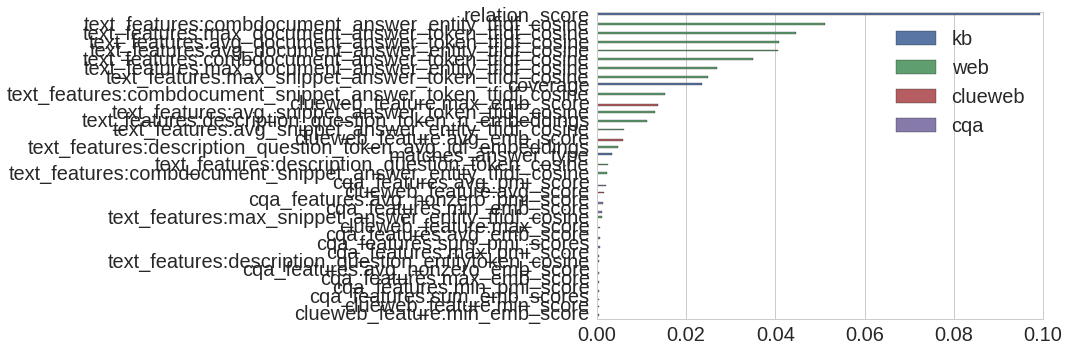
\includegraphics[width=\textwidth]{img/feature_importances}
\caption{Importances of different text-based features for KBQA (features with * are not text-based and are provided for comparison)}
\label{fig:feature_importances}
\end{figure*}

The figure supports the observation that web search results based features turned out to be the most useful among other text-based data sources.
However, other text data sources also contribute to the overall improvement.
According the model, best feature based on entity pair language model computed on ClueWeb dataset is more useful than CQA-based features.

\section{Analysis and Discussion}
\label{section:analysis}
% We have shown that Text2KB outperforms the baseline.
We now investigate how our system would compare to other systems on the same benchmark; then, we investigate in depth the different error modes (Section \ref{section:analysis:error}), which helps identify the areas of most substantial future improvements. 

\begin{table}
\centering
\caption{Average Recall (R), Precision (Pr), and F1 for Text2KB (our system), STAGG and their combinations}
\label{table:combine_stagg}
\begin{tabular}{| p{4cm} | p{1cm} | p{1cm} | p{1cm} | }
\hline
System & R & P & F1 \\
\hline
%Aqqu (baseline) \cite{ACCU:2015} & 0.604 & 0.498 & 0.494\\
% DIDN'T HAVE TIME TO IMPLEMENT THIS.
% Text-only baseline & & & & \\
Our system: Text2KB & 0.6354 & 0.5059 & 0.5223 \\
STAGG \cite{yih2015semantic} & 0.607 & 0.528 & 0.525\\
\hline
Text2KB + STAGG & 0.5976 & 0.5343 & 0.5320 \\
Text2KB + STAGG (oracle) & 0.7144 & 0.5904 & 0.6056 \\
\hline
\end{tabular}
\end{table}

We took an existing KBQA systems and demonstrated that by combining evidence from knowledge base and external text resources we can boost the performance.
A reasonable question is whether the same approach will be helpful to other systems, \eg the currently best system -- STAGG \cite{yih2015semantic}.
STAGG differs from our baseline system Aqqu in the components: entity linking algorithm, a set of query templates and ranking methods.
Therefore, our approach is complementary and should be helpful for STAGG as well.
To support this claim, we made an experiment to combine answers of STAGG and Text2KB.
One of the advantages of the former is its set of filters, that restricts list results to entities of certain type, gender, \etc
Therefore, we combined answers of STAGG and Text2KB using a simple heuristic: we chose to use the answer returned by STAGG if the number of answer entities is less than in the Text2KB answer, otherwise we use the answer of our approach.
Table \ref{table:combine_stagg} gives the results of the experiment, and as we can see the combination achieves slightly a better average F1 score.
Alternatively, we can look at the oracle combination of the systems, which always selects the answer with higher F1, which demonstrate that systems don't make exactly the same mistakes and therefore can be combined.
As we can see such a combination results in a performance of 0.6056, which is much higher than either of the systems.

As we mentioned earlier, answers to 112 of the test questions in WebQuestions dataset involve a predicate that weren't observed in the training set, which may be a problem for approaches that rely on a trained lexicon.
We evaluated both systems on these questions, and indeed the performance is very low, \ie the average F1 score of Text2KB is 0.1640 compared to 0.1199 for STAGG\footnote{Unfortunately, the number of questions is too low to show statistical significance (p-value=0.16)}.

\subsection{Error analysis}
\label{section:analysis:error}

\begin{figure}
\centering
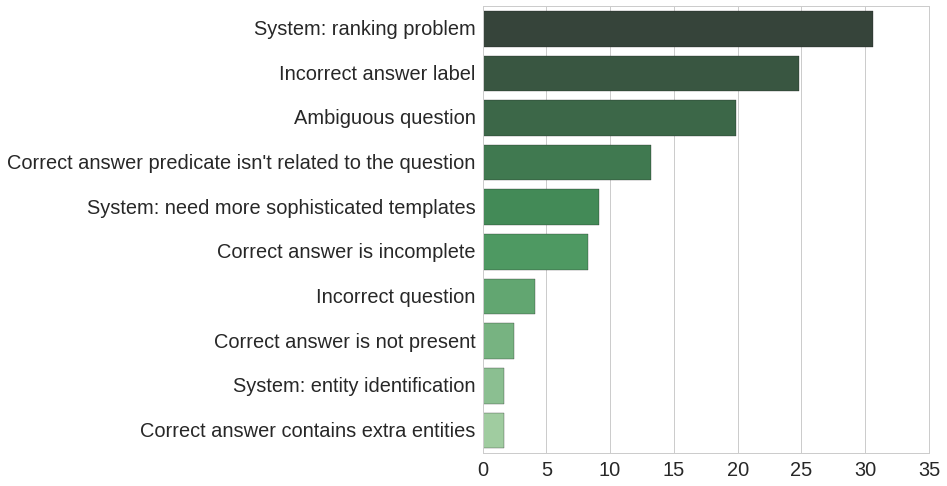
\includegraphics[width=0.45\textwidth]{img/error_analysis}
\vspace{-0.5cm}
\caption{Distribution of problems with questions, where Text2KB returns an answer with F1$<$1}
\label{fig:error_analysis}
\vspace{-0.3cm}
\end{figure}

To get a better insights into the problems that remain, we collected 1219 questions for which Text2KB didn't return completely correct answer, \ie F-1 score $<$ 1.
We manually looked through a couple of hundreds of these examples and grouped the problems into several clusters (Figure \ref{fig:error_analysis}).

As we can see candidate ranking is still the major problem, and it accounts for $~31\%$ of the cases.
The second most popular problem is incorrect ground truth labels (almost a quarter of errors).
For example: for the question \textit{when tupac was shot?''} the label says \texttt{Tupac 1994 assault} instead of \texttt{Las Vegas}.
Another set of questions have incomplete or overcomplete ground truth answer list.
Typical examples are questions asking for a list of movies, books, landmarks, \etc
The ground truth answer usually contains $\sim10$ entities, whereas the full list is often much larger.
This seems to be an artifact of the labeling process, where the answer was selected from the Freebase entity profile page, which shows only a sample of 10 entities, while the rest is hidden behind the ``NNN values total'' link.
About 20\% of the questions are ambiguous, \ie questions have no strict 1-1 correspondence with any of the predicates and can be answered by multiple ones without any obvious preferences.
% for the question \textit{``where is shakira from?''} the ground truth is the country - \texttt{Colombia}, while Text2KB returned her place of birth - \texttt{Barranquilla}.
For example, the question \textit{``what did hayes do?''} can be answered by profession, occupied position or some other achievements.
Another problem is when there is no predicate that answers the question.
For example, the question \textit{``what do people in france like to do for fun?''} doesn't have a good match among the facts stored in Freebase.
The ground truth entity \texttt{Cycling} comes from the list Olympic sport competitions country participated\footnote{\texttt{olympics.olympic\_participating\_country.athletes}}.
% In some cases there are entities that are very similar in meaning, but represented in Freebase by different ids and names.
% For example, the answer to the question \textit{``what is william taft famous for?''} is \textit{``President of the United States''}, which is a government position, but there is also a triple \texttt{[William Howard Taft, common.topic.notable\_for, US President]}, where the last entity represents a type of people who help the position, and is considered incorrect.

% This is nice, but probably is too little to mention.
% We also noticed, that in a small number of examples, the case of the correct answer entity and the answer returned by the system is different.
% For example, for the question \textit{``what fma stands for?''} the correct answer specified in the dataset is \textit{``FullMetal Alchemist''}, while the actual name of the entity is \textit{``Fullmetal Alchemist''}.
% The official evaluation script don't normalize the case and therefore considers this example incorrect.
% If we lowercase all entity names before comparison, the average F1 score of Text2KB becomes 0.5248.

Text2KB components were quite effective in resolving some of the problems.
Web search results helped identify the right question topical entity in a number of cases, \eg \textit{``what did romo do?''} mentions only the last name of the Dallas Cowboys quarterback and the baseline system were unable to map it to the right entity.
Web search results provides more than enough evidence that romo refers to \texttt{Tomo Romo}.
However, there are a number of loses, introduced by added unrelated entities.
For example, the entity \texttt{I Love Lucy} was added for the question \textit{``what was lucille ball?''}, because the term \textit{lucy} had high similarity with \textit{lucille}.
A portion of these problems can be fixed by a better entity linking strategy, \eg \cite{SMAPH_ERD:2014}.
An interesting example, when external text resources improved the performance is the question \textit{``what ship did darwin sail around the world?''}.
This is actually a hard question, because the ship entity is connected to the \texttt{Charles Darwin} entity through the ``knownFor'' predicate along with some other entities like \texttt{Natural selection}.
% \footnote{\texttt{user.lindenb.default\_domain.scientist.known\_for}
Thus, the predicate itself isn't related to the question, but nevertheless, the name of the ship \texttt{HMS Beagle} is mentioned multiple times in the web search results, and entity pair model computed from ClueWeb also has high scores for the terms ``ship'' and ``world''.

There are several major reasons for the loses, introduced by features based on external text resources.
Some entities often mentioned together and therefore one of them gets high values of cooccurrence features.
For example, the baseline system answered the question \textit{``when did tony romo got drafted?''} correctly, but since \texttt{Tony Romo} is often followed by \texttt{Dallas Cowboys}, Text2KB ranked the team name higher.
Another common problem with our features is an artifact of entity linking, which works better for names and often skips abstract entities, like professions.
For example, the correct answer to the question \textit{``what did jesse owens won?''} is an entity with the name \texttt{Associated Press Male Athlete of the Year}, which is rarely mentioned or it's hard to find such mentions.
Some problems were introduced by a combination of components.
For example, for \textit{``where buddha come from?''} a topical entity \texttt{Buddhism} was introduced from search results, and it generated \texttt{Gautama Buddha} as one of the answer candidates.
This answer was ranked the highest due to large number of mentions in the search results.

In summary, we show that ideas behind Text2KB could be integrated into other systems and improve their performance.
The error analysis suggested that even though a significant number of questions in the WebQuestions dataset have incorrect or ambiguous ground truth labels, there is still a room for improvement.
In particular, the future work for Text2KB will include a better strategy for entity linking using external data sources and a better context model for entity mentions in text documents, which can put more weight on entities mentioned in the context related to the question.


\section{Related Work}
\label{section:related_work}

Recent development of large scale knowledge bases (e.g. dbPedia \cite{auer2007dbpedia}) and Freebase \cite{Bollacker:2008:FCC:1376616.1376746}) motivated research in open domain question answering over linked data.

In 2011 a series of QALD (Question Answering over Linked Data) evaluation campaigns has started, report on the last one, QALD-5, can be found in \cite{UngerFLNCCW15}.
These benchmarks target dbPedia as a knowledge base and provide a rather small (50-350) training set of questions, annotated with correct SPARQL queries.
In QALD-3 a multilingual task has been introduced, and since QALD-4 it includes the hybrid task, that asks participants to build systems that can use both structured data and free form text available in dbPedia abstracts.
The formulation of the hybrid task is the most relevant to our work, however, there are a couple of key differences: unlike this work the hybrid task questions are manually created so that they could \emph{only} be answered by combining RDF and text data.
The second difference lies in the nature of text data used for question answering.
In this work we use a broad spectrum of various text resources, such as web search results, CQA archives and semantically enriched text documents, while the focus of the task is on relatively short abstracts.
Lastly, because of the expensive labeling process QALD datasets are small, for example, QALD-5 training set for multilingual question answering included 300 examples and hybrid - 40 examples (the evaluation was done on 50 questions for multilingual task and just 10 for hybrid).
The scale of the datasets makes it hard to use machine learning, which lies in the heart of this work.
For these reasons, we didn't include QALD in our evaluation experiments.
However, we acknowledge the importance of QALD and intend to look into it and especially into the hybrid track in the future.

WebQuestions benchmark dataset was developed in \cite{Berant:EMNLP13} and since triggered a number of works that explored both semantic parsing and information extraction approaches for KBQA \cite{yao2014freebase}.
Developed system differ in ways question entity is detected, candidate answers are generated, features used and the answer is selected.
The most interesting aspect for this work is the use of external resources, that help translate natural language text into KB properties and entities.
Such a lexicon can be learned from a labeled training set \cite{Berant:EMNLP13},  ClueWeb collection aligned to Freebase \cite{yao2014information}, question paraphrases clusters from WikiAnswers \cite{berant2014semantic}, Freebase triples rephrased as questions \cite{BordesCW14:emnlp}, and can be based on the embeddings of questions and knowledge base entities and predicates \cite{BordesCW14:emnlp,yih2015semantic}.
However, most of the models are still biased towards the types of questions present in the training set and would benefit from more training data.
In this work I propose to extend the training set with question-answer pairs available on CQA websites, which were shown to be useful for relation extraction \cite{savenkov-EtAl:2015:SRW}.
In addition, I propose to use unlabeled text resources for candidate query ranking, which can help to generalize to unseen types of questions and questions about predicates never mentioned in the training set.

In general, combination of different data sources, such as text documents and knowledge bases, for question answering is not a novel idea and it has been already implemented in hybrid QA systems \cite{baudivs2015modeling}, \eg IBM! Watson combined text and structured data resources in their Jeopardy! winning system \cite{Barker12}.
The key difference of our approach is that such hybrid systems typically have separate pipelines to generate candidate answers from different data sources and only rank them together to select the best one.
In this work we attempt to integrate text resources inside the KBQA answer generation and scoring.

Another interesting attempt to combine the data sources has been made by  \cite{Sun:2015:ODQ:2736277.2741651}, who showed that entity types and descriptions can be effectively used by text-based question answering systems.
In this work, we focus on the inverse problem of improving knowledge base question answering by incorporating natural language text resources.
..... MENTION JEFF DALTON'S WORK ON ENTITY ENRICHMENT \cite{dalton2014entity}.

Open IE extractions \cite{fader2011identifying} represent an interesting mixture between text and structured data and can be considered as an intermediate step between raw text and structured KB.
Such knowledge repositories can be queried using structured query languages such as SPARQL and at the same time allows text matching against entities as predicates.
One can easily transform an existing KB to such a form by replacing predicates and entities with their names and  \cite{Fader:2014:OQA:2623330.2623677} demonstrated that even though such an approach looses to existing baselines on WebQuestions dataset, where questions are known to be answerable from KB, achieves higher scores on TREC and WikiAnswers benchmarks.


\section{Conclusions and Future Work}

Our work showed that unstructured text resources can be effectively utilized for knowledge base question answering to improve query understanding,  candidate answer generation and ranking.
We focused on three particular techniques and associated text information sources: web search results for query understanding and candidate ranking, community question answering data for candidate generation, and text fragments around entity pair mentions for ranking. Certainly, there are more resources that could be potential adapted, \eg entity profile pages like Wikipedia, news sources, textbooks, and many others. However, we believe that the proposed approach is general enough that it could be extended and successfully incorporate these other diverse text sources.

In the future, we plan to extend our work to the more open setup, similar to the QALD hybrid task, where questions no longer have to be answered exclusively from the KB. This would require extending the described techniques, and creating new QA benchmarks.



%ACKNOWLEDGMENTS are optional
%\section{Acknowledgments}
%Thanks to anonymous reviews for accepting this paper.

%
% The following two commands are all you need in the
% initial runs of your .tex file to
% produce the bibliography for the citations in your paper.

\vspace{1.0cm}
\bibliographystyle{abbrv}
\bibliography{sigproc}  % sigproc.bib is the name of the Bibliography in this case
% You must have a proper ".bib" file
%  and remember to run:
% latex bibtex latex latex
% to resolve all references
%
% ACM needs 'a single self-contained file'!
%
%APPENDICES are optional
%\balancecolumns
% \appendix
%Appendix A

\end{document}
